\begin{frame}
	\frametitle{Local elections 2014 - results summary}
	\begin{itemize}
	\item \textbf{Marienbad}: 4 Pirates, majority with 21\%
	\item \textbf{Prague}: 4 Pirates at city council (5,31\%), 7 Pirates in districts
	\item Brno: 2 Pirates 11,88\% (coalition - \v{Z}\'it Brno movement)
	\item Majet\'in: 1 Pirate
	\item Prost\v{e}jov: 1 Pirate (coalition)
	%% \item \v{S}umperk 1 independent (coalition)
	%% \item Olomouc (coalition) - Pirate didn't get a seat, possi
	%% \item P\v{r}erov (coalition) - 
	%% \item Jesen\'ik (pseudocoalition - Pirates under greens)
	\item St\v{r}\'ibro: 1 Pirate
	\item Trutnov: 1 Pirate
	%% \item Liberec 2 independent
	\item P\'isek: 1 Pirate
	\item Kralupy nad Vltavou: 1 Pirate
	\item Sadsk\'a: 1 Pirate (coalition)
	\item many independent candidates under Pirate flag
\end{itemize}
\end{frame}
\begin{frame}
	\frametitle{Marienbad}
	\begin{itemize}
	\item 5 mandates, 4 Pirates \& 1 independent, majority with 21\%
	\item Vast policy, clearly commenting on local issues
	\item Trustworthy candidates with long-term activity record
	\item PR newspaper distributed to every mailbox in the city
	\item Main policies presented in articles
	\item Posters with slogans
	\item Website pirati.ml, social network activity
	\item Local VyOseni, underground art community
	\item Incapability of other politicians in the city
	\item History of success: 2012 - 5,50\%, 2013 - 5,85\%, 2014 - 8,50\%
	\end{itemize}
	%%http://www.piratiml.cz/download/Piratske_listy_marianskolazenske_2014.pdf
\end{frame}
\begin{frame}
	\frametitle{Prague}
	\begin{itemize}
		\item 4 Pirates at city council + 7 Pirates \& 5 supporters in districts
		\item Leader, known as information freedom activist
		\item PR newspaper distributed around busy underground stations
		\item PR happenings
		\item History of success
		\item Budget, regular meetings, started right after EP elections
		\item Big effort of many volunteers and candidates
		\item Policy focused on local issues
		\item Logo
		\item prahavolijinak.cz website
	\end{itemize}
\end{frame}
\begin{frame}
	\frametitle{Prague - logo}
	\begin{center}
	\begin{multicols}{2}
		
\includegraphics[width = 0.38\textwidth]{Praha.eps}
		
		
\includegraphics[width = 0.38\textwidth]{logo_pirati.eps}
	\end{multicols}
	\end{center}
\end{frame}
\begin{frame}
	\frametitle{Prague - newspaper}
	\begin{center}
	\begin{multicols}{2}
		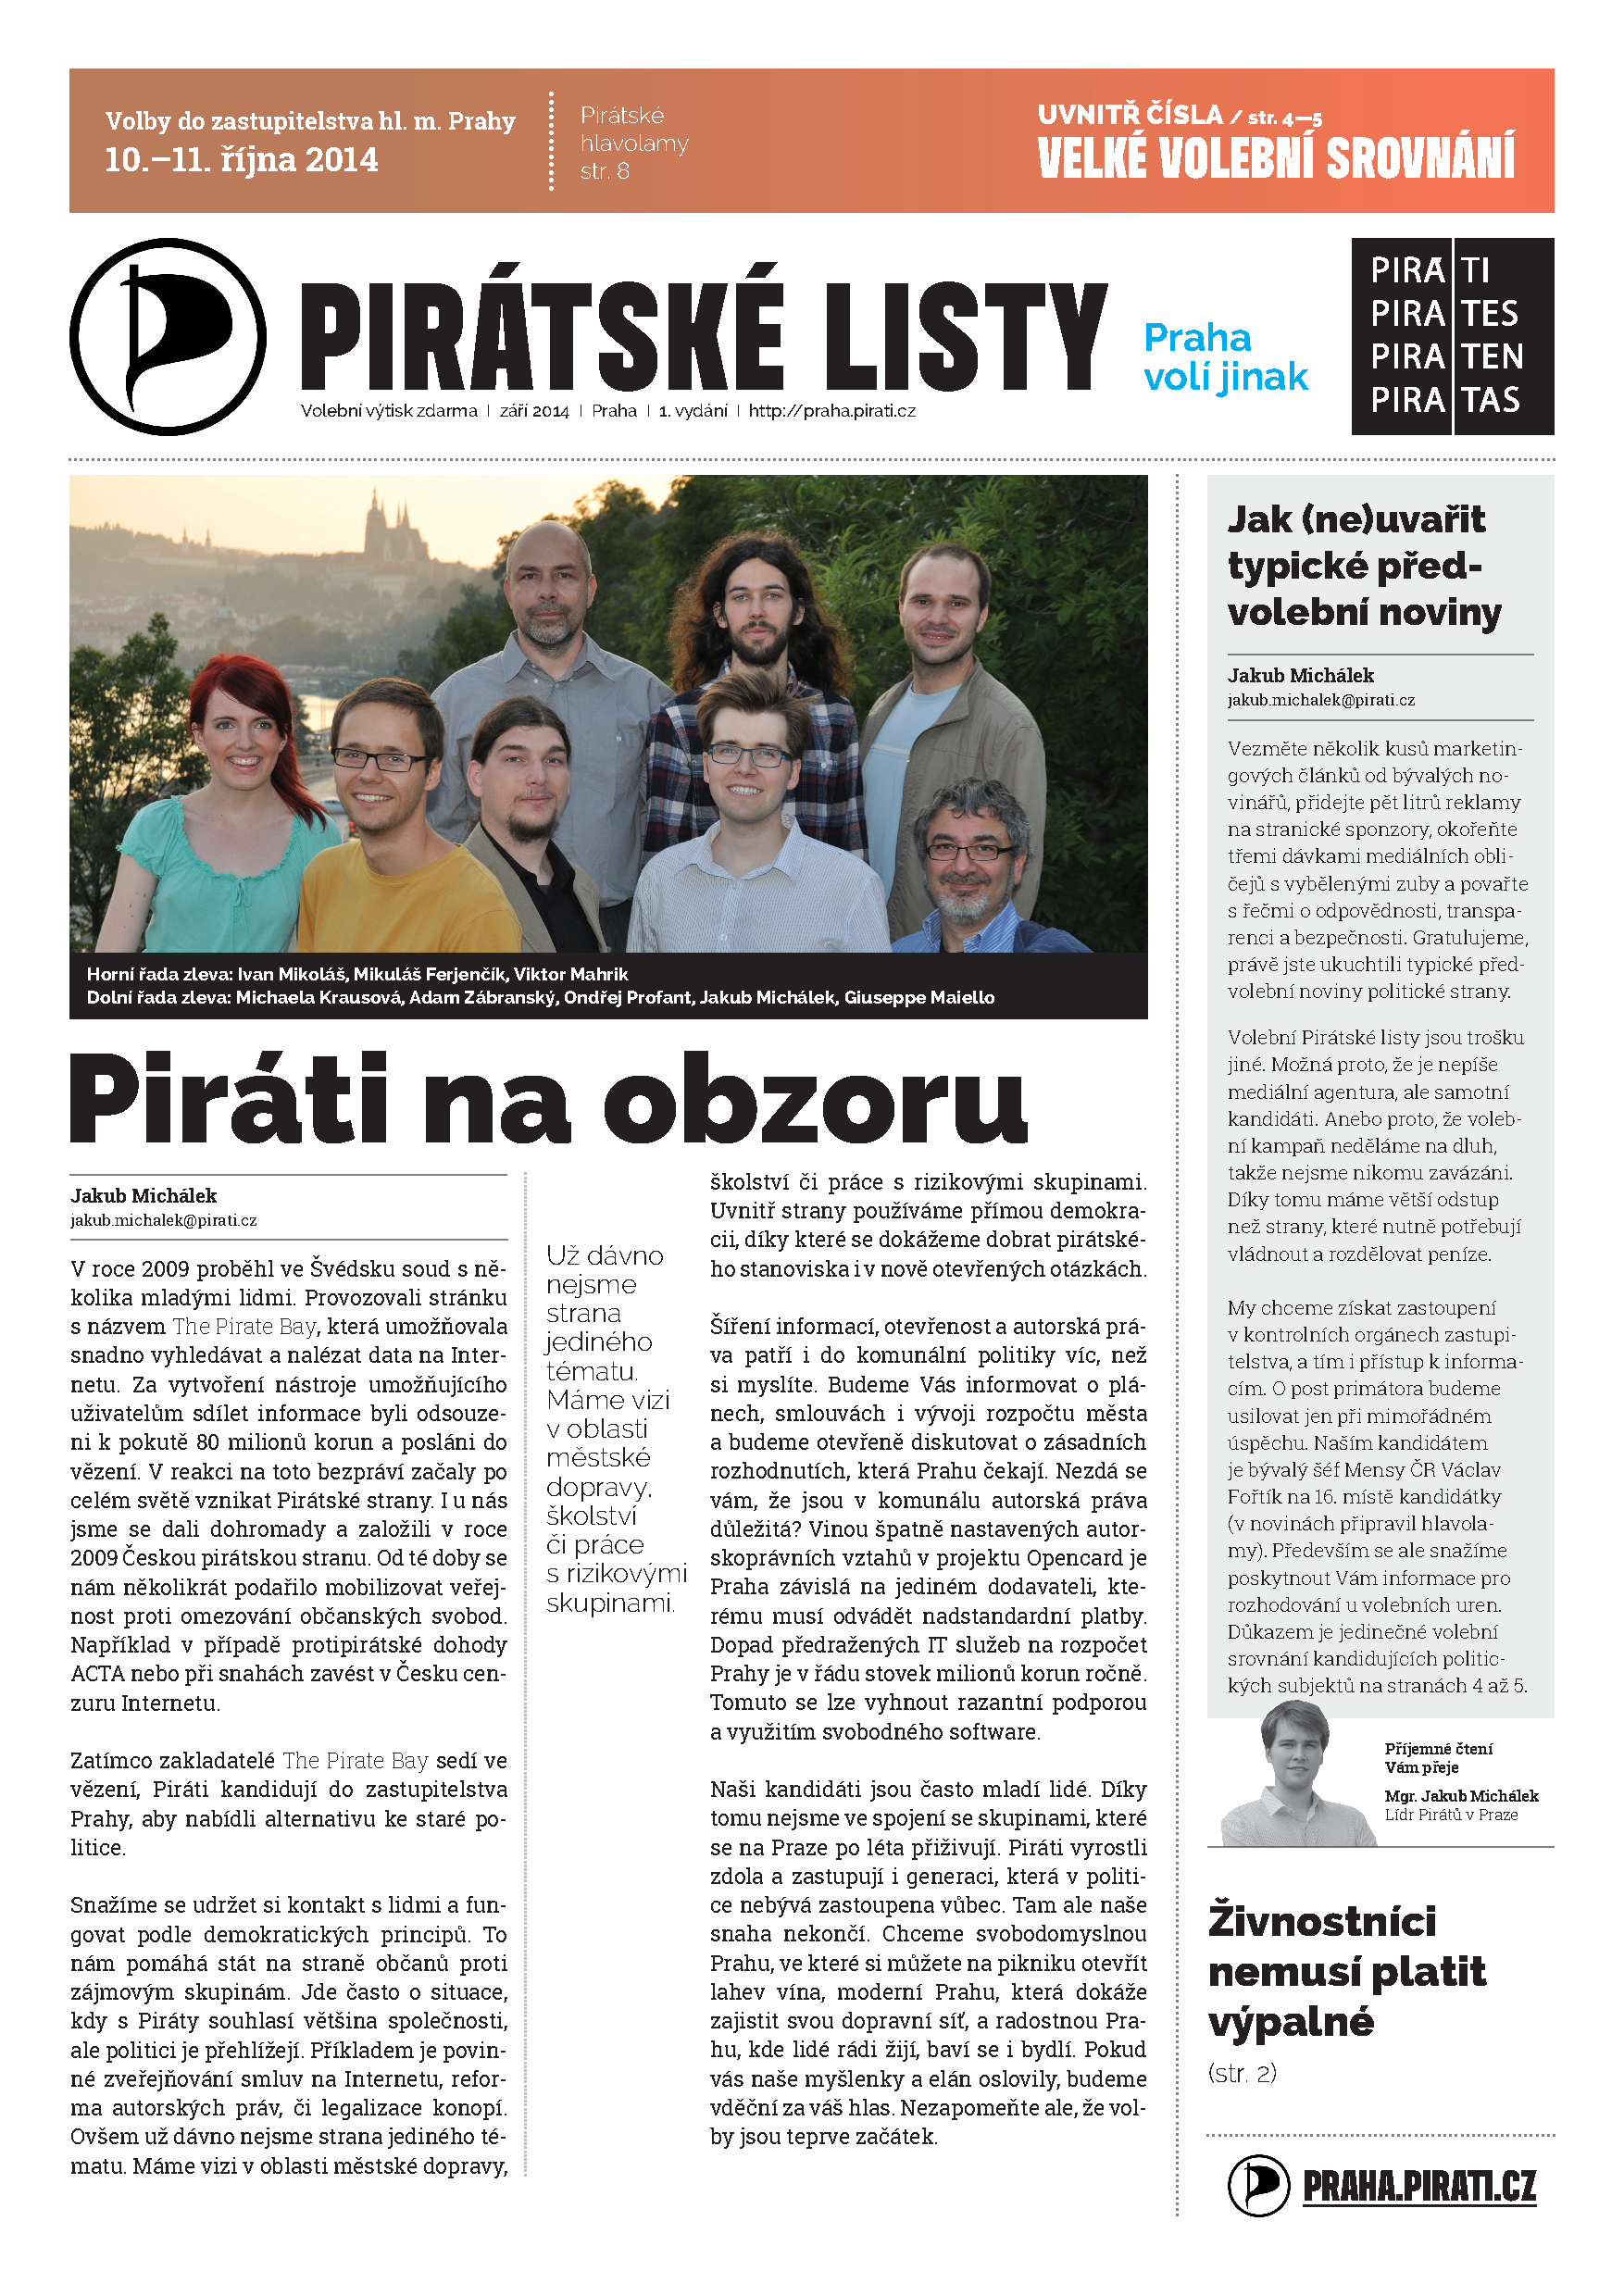
\includegraphics[width = 0.45\textwidth]{listy1.pdf}
		
		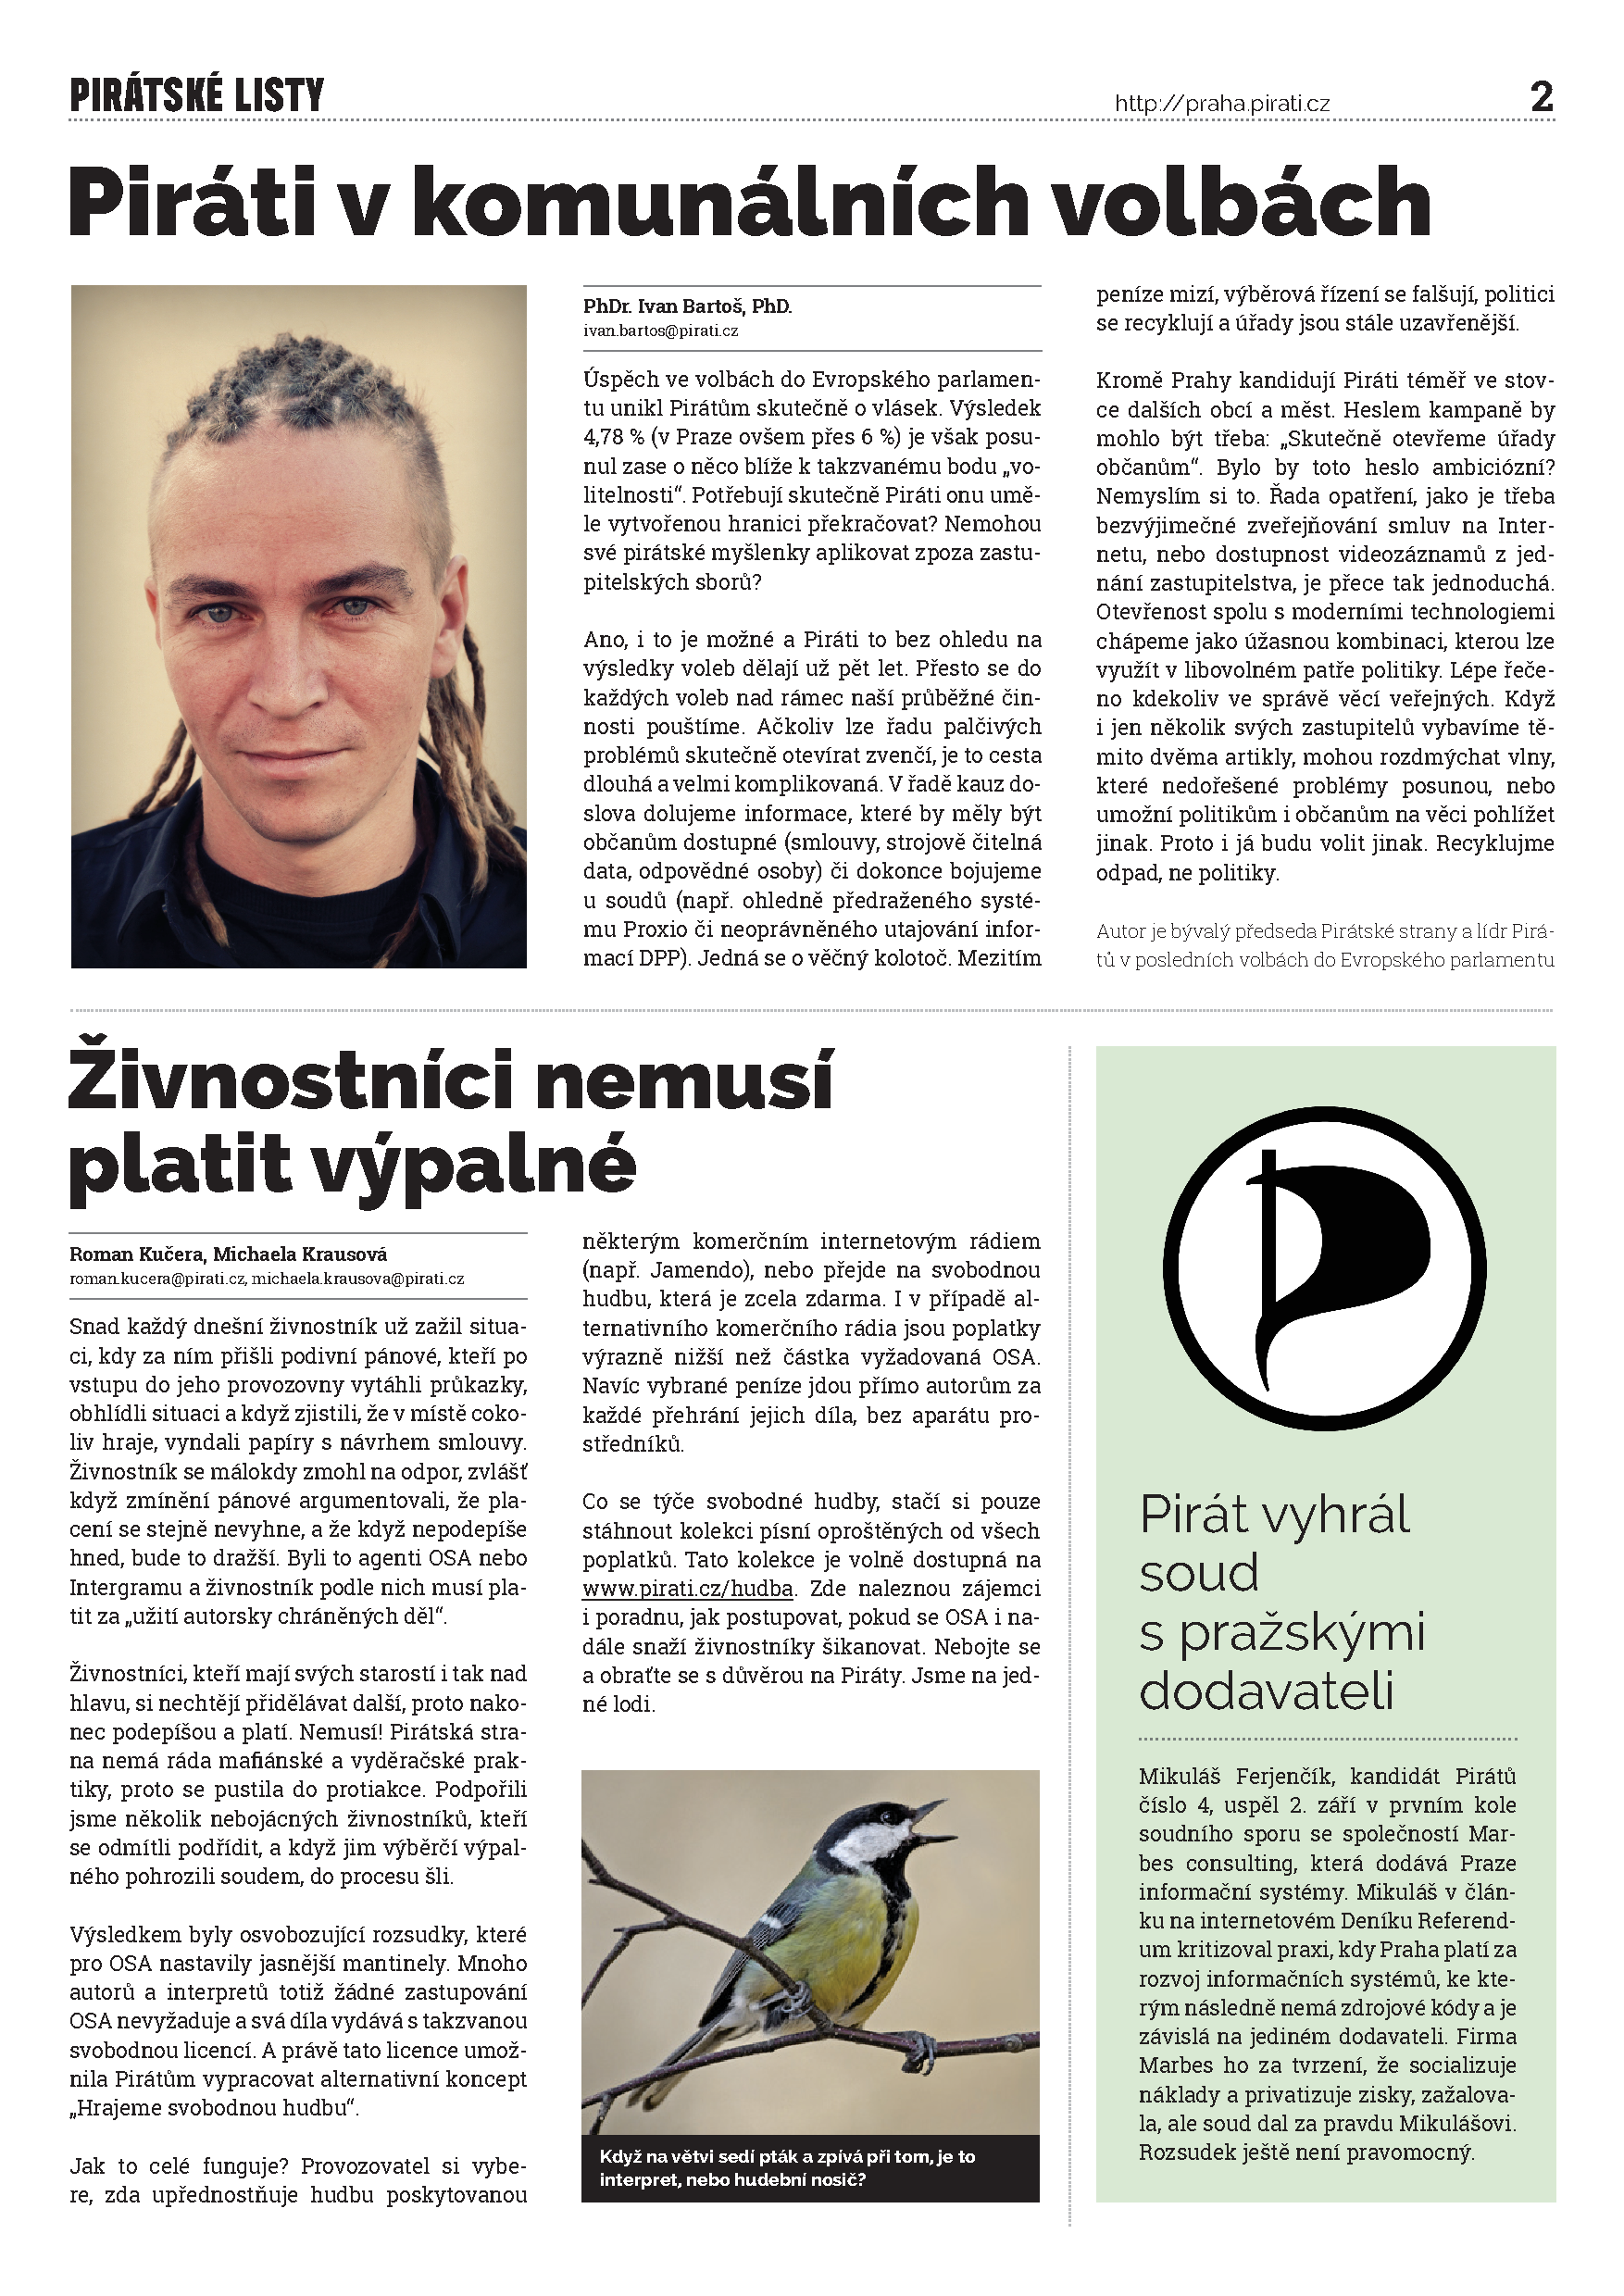
\includegraphics[width = 0.45\textwidth]{listy2.pdf}
	\end{multicols}
	\end{center}
\end{frame}
\begin{frame}
	\frametitle{Brno}
	\begin{itemize}
		\item \v{Z}\'it Brno movement
		\item 11,88\%, 2 pirates
		\item First - recesistic movement criticizing local mayor
		\item When got FB page blocked, wider group of local activists formed
		\item Young green liberal hipsters who want better city
		\item Representatives of several citizen's initiatives and Pirate party
	\end{itemize}
\end{frame}
\begin{frame}
	\frametitle{Notes \& experience}
	\begin{itemize}
		\item Election system allows "preferential votes"
		\item Often happened that in coalitions Pirate candidates were "outvoted" on lower positions
		\item Better poll attendance of coalition partners voters etc.
		\item Better to stay independent
	\end{itemize}
\end{frame}
\begin{frame}
	\frametitle{General policy for communal elections}
	\begin{itemize}
		\item Vast document covering all sort of issues
		\item Transformed into local policies reflexing local issues
		\item Economy - transparent, balanced, effective
		\item Participation - open access, support active citizens
		\item Public service for citizens - traffic infrastructure
		\item Modern technology - dealing with state, free formats, internet access
		\item Investiotions into education and culture
		\item Available health and social services
		\item Environment protection
	\end{itemize}
\end{frame}
\begin{frame}
	\frametitle{After elections - general strategy}
	\begin{itemize}
		\item Piratecon - improve qualification
		\item How to be a good representative
		\item How to introduce free software and OpenData
		\item How to assign work to officers
		\item YOU'RE WELCOME TO VISIT
	\end{itemize}
\end{frame}
\begin{frame}
	\frametitle{Summary - how to score}
	\begin{itemize}
		\item constant activity for people
		\item wide policy focused on the location
		\item clean image
		\item cooperation across the Party \& international
	\end{itemize}
\end{frame}
